\documentclass{exam}
\usepackage{main}
\qformatExam{}

\title{Devoir sur table}
\date{30 Novembre 2023}
\author{}

\begin{document}
\maketitle

\begin{itemize}
\item L'usage de la calculatrice est INTERDIT.
\item Tout effort de recherche, même s'il n'aboutit pas, sera valorisé.
\item Une bonne présentation est exigée, et sera notée sur 2 points.
\end{itemize}
\vspace*{0.5cm}
\begin{questions}
\titledquestion{Sommes de vecteurs}[5]
Tous les triangles tracés sur la figure sont des triangles équilatéraux. \emph{Il n'est pas nécessaire de faire des phrases pour justifier vos réponses dans cet exercice.}
\begin{center}    
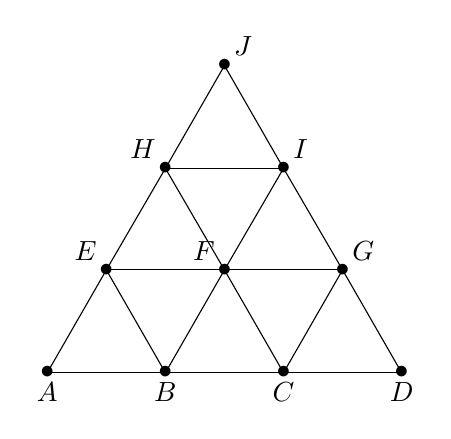
\begin{tikzpicture}[scale=1.5]
\coordinate (A) at (0,0);
\coordinate (B) at (1,0);
\coordinate (C) at (2,0);
\coordinate (D) at (3,0);
\coordinate (E) at (0.5,0.87);
\coordinate (F) at (1.5,0.87);
\coordinate (G) at (2.5,0.87);
\coordinate (H) at (1,1.73);
\coordinate (I) at (2,1.73);
\coordinate (J) at (1.5,2.60);

\draw (A) -- (B) -- (C) -- (D);
\draw (E) -- (F) -- (G);
\draw (H) -- (I);
\draw (A) -- (E) -- (B) -- (F) -- (C) -- (G) -- (D);
\draw (E) -- (H) -- (F) -- (I) -- (G);
\draw (H) -- (J) -- (I);
\draw (A) node {$\bullet$} node[below] {$A$};
\draw (B) node {$\bullet$} node[below] {$B$};
\draw (C) node {$\bullet$} node[below] {$C$};
\draw (D) node {$\bullet$} node[below] {$D$};
\draw (E) node {$\bullet$} node[above left] {$E$};
\draw (F) node {$\bullet$} node[above left] {$F$};
\draw (G) node {$\bullet$} node[above right] {$G$};
\draw (H) node {$\bullet$} node[above left] {$H$};
\draw (I) node {$\bullet$} node[above right] {$I$};
\draw (J) node {$\bullet$} node[above right] {$J$};
\end{tikzpicture}
\end{center}
Répondre aux questions suivantes :
\begin{parts}
\part Citer deux vecteurs égaux au vecteur $\vect{EF}$.
\part Quelle est l'image du point $H$ par la translation de vecteur $\vect{CG}$ ?
\part Citer le représentant de $\vect{BE}$ d'origine $I$.
\part Compléter les égalités vectorielles suivantes à l'aide d'un seul vecteur entre deux points de la figure :
\begin{equation*}
\begin{aligned}
\vect{AB} + \vect{BC} = \dots\\
\vect{GC} + \vect{EF} = \dots\\
\vect{HI} + \vect{BA} = \dots\\
\vect{BC} + \vect{FG} + \vect{EH} = \dots\\
\end{aligned}
\end{equation*}
\end{parts}
\vspace*{0.5cm}
\titledquestion{Sommes de vecteurs}[5]
Soient $A$, $B$ et $I$ trois points du plan non alignés. On pose $C$ tel que $\vect{AI} = \vect{IC}$, et $D$ tel que $\vect{BI} = \vect{ID}$.
\begin{parts}
\part Faire une figure.
\part Justifier en une phrase que $\vect{AB} = \vect{AI} + \vect{IB}$.
\part En déduire que $\vect{AB} = \vect{DC}$.
\part Conclure que le quadrilatère $ABCD$ est un parallélogramme.
\end{parts}
\vspace*{0.5cm}
\titledquestion{Repère orthonormé}[5]
On donne une représentation d'un repère orthonormé $(O;I;J)$.
\begin{center}
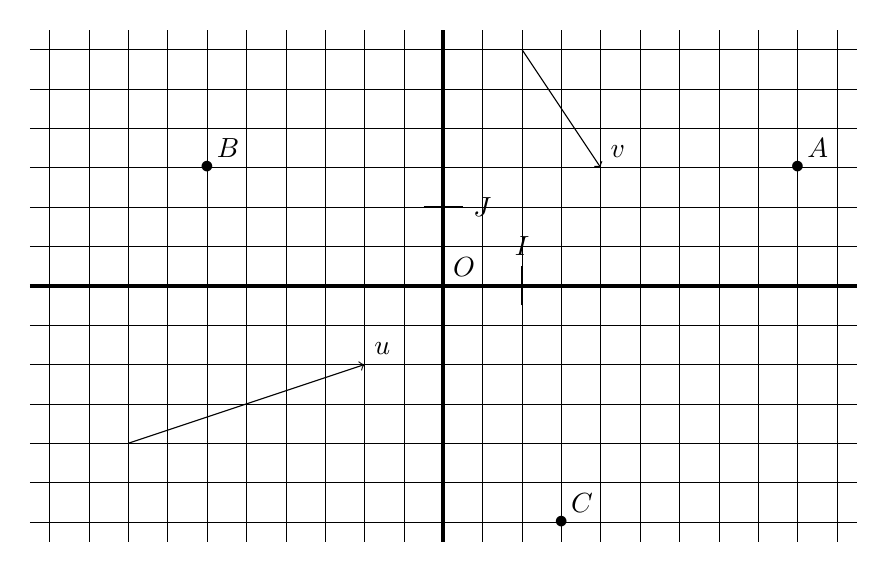
\begin{tikzpicture}
\draw[very thin] (-5.25,-3.25) grid[step=0.5] (5.25,3.25);
\draw[ultra thick] (-5.25,0) -- (5.25,0);
\draw[ultra thick] (0,-3.25) -- (0,3.25);
\draw (0,0) node[above right] {$O$};
\draw[thick] (1,-0.25) -- (1,0.25) node[above]{$I$};
\draw[thick] (-0.25,1) -- (0.25,1) node[right]{$J$};

\draw (4.5,1.5) node {$\bullet$} node[above right] {$A$};
\draw (-3,1.5) node {$\bullet$} node[above right] {$B$};
\draw (1.5,-3) node {$\bullet$} node[above right] {$C$};

\draw[->] (-4,-2) -- (-1,-1) node[above right] {$\vect{u}$};
\draw[->] (1,3) -- (2,1.5) node[above right] {$\vect{v}$};
\end{tikzpicture}
\end{center}
\begin{parts}
\part En nombre de carreaux, quelle est la longueur d'une unité dans ce repère ?
\part Par lecture graphique, donner les coordonnées de $A$, $B$ et $C$ dans ce repère.
\part Par lecture graphique, donner les coordonnées des vecteurs $\vect{AB}$, $\vect{CB}$, $\vect{u}$ et $\vect{v}$ dans ce repère.
\part Tracer sur ce repère un représentant du vecteur $\vect{w} = \vect{u} + \vect{v}$.
\part Tracer sur ce repère un représentant du vecteur $-\vect{v}$.
\end{parts}
\vspace*{0.5cm}
\titledquestion{Coordonnées de vecteurs}[5]
Cet exercice ne nécessite pas de dessiner un repère. Soit $(O;I;J)$ un repère orthonormé, et $A(6;1)$, $B(5;-8)$, $C(9;-3)$. On pose $M(x;y)$ tel que $\vect{AM} = \vect{AB} + \vect{AC}$.
\begin{parts}
\part Calculer les coordonnées des vecteurs $\vect{AB}$ et $\vect{AC}$.
\part En déduire par le calcul les coordonnées de $\vect{AB} + \vect{AC}$.
\part Exprimer les coordonnées de $\vect{AM}$ en fonction de $x$ et de $y$.
\part En déduire les coordonnées de $M$.
\end{parts}
\vspace*{0.5cm}
\titledquestion{Bonus}[2]
On définit le \emph{double} d'un vecteur $\vect{u}$, noté $2\vect{u}$, par un vecteur de même direction et de même sens que $\vect{u}$, mais de norme doublée.
Dessiner un repère orthonormé $(O;I;J)$, représenter le vecteur $\vect{u}$ d'abscisse $2$ et d'ordonnée $3$, puis représenter le vecteur $2\vect{u}$. Par lecture graphique, quelles sont les coordonnées de $2\vect{u}$ ?
\end{questions}
\end{document}